\chapter{Approach}
\todo{Why are we using a data-driven / machine learning approach? Show that it is complicated to do it by hand. Also write why not to do auto-tuning.}

\begin{figure}
    \centering
    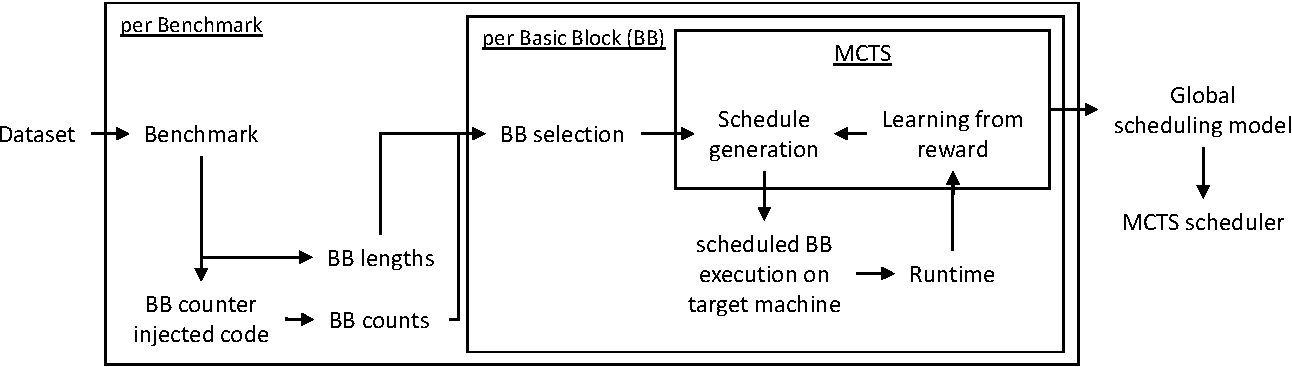
\includegraphics[width=\textwidth]{img/ppt/approach_overview-crop.pdf}
    \caption[Overview of the approach]{Overview of the overall approach. 
    The process covers the selection of basic blocks, the instruction schedule generation, the execution model, the learning process and the derivation of the final scheduler.}
    \label{fig:approach:overview}
\end{figure}
In the rest of this chapter, we present the approach used for this thesis (compare~\cref{fig:approach:overview}).
We start with an overview of the benchmark programs we used~(\cref{sec:approach:dataset}).
Then we discuss the importance of basic blocks for instruction scheduling in general and our approach specifically~(\cref{sec:approach:basicblock}).
That is followed by explaining the \ac{mcts} approach~(\cref{subsec:approach:ml:mcts}).
Eventually, we introduce our approach for combining individual \ac{mcts} models into a global model~(\cref{subsec:approach:ml:global}) and derive an applicable scheduler~(\cref{sec:approach:ml-scheduler}).

\section{Dataset}
\label{sec:approach:dataset}
For our experiments, we use benchmarks from the LLVM project~\cite{LLVM:CGO04} called LLVM Test Suite~\footnote{\url{https://llvm.org/docs/TestSuiteGuide.html}}.
The test suite contains benchmarks from the following categories
\begin{itemize}
    \item Single-Source --- built from a single C/C++ source file
    \item Multi-Source --- built from multiple C/C++ source files
    \item Micro-Benchmarks --- separate functions that are executed by google-benchmark
    \item Bitcode --- tests that are written in LLVM bitcode
    \item CTMark --- symbolic links to the other benchmarks to measure compilation performance
\end{itemize}
We select the 273 benchmarks from the Single-Source and Multi-Source categories for our experiments.
\todo{Add table?}
These categories contain benchmarks that are compiled from a single source file or multiple source files, respectively.
The benchmarks are all written in C or C++.
In addition, the test suite contains more benchmarks that are not relevant to our experiments. \todo{Why not?}

\subsection{Modified Build Process}
\label{sec:approach:build_process}
The test suite comes with Makefiles and CMake configurations to automatically build all benchmarks.
However, these are not sufficient for our approach.
We need a modified build process for all the benchmarks because we are manipulating it in several cases.
Furthermore, the compilation cannot be done by a single command because not all arguments of the separate compilation steps are available in the main compiler.
We execute the front-end, optimization, and back-end compiler phases separately to have complete control over the build process.

We have to set some compiler arguments to make the LLVM compiler front-end output LLVM \ac{ir} instead of compiling the program to an executable format.
We use the compiler \lstinline{clang}~\footnote{\url{https://clang.llvm.org/}} for C programs and \lstinline{clang++} for C++ programs
However, the compiler arguments are the same.
We pass the following arguments to the front-end:
\begin{itemize}
    \item \lstinline{-O0}: to prevent optimization in this first step
    \item \lstinline{-Xclang -disable-O0-optnone}: the \lstinline{-O0} flag alone also prevents optimization in further steps, which is not what we want
    \item \lstinline{-S -emit-llvm}: to emit LLVM \ac{ir} for further processing --- instead of compiling the program completely
\end{itemize}

The LLVM optimizer \lstinline{opt}~\footnote{\url{https://llvm.org/docs/CommandGuide/opt.html}} gives a choice to select one of the predefined optimization levels or select specific optimizer runs.
When we compile a benchmark for measuring the runtime, we only use the flag \lstinline{-O3} for optimizing the LLVM \ac{ir}.
The LLVM framework makes it easy to implement new optimizer passes.
We do this to count how often a basic block is executed (see \cref{sec:approach:basicblock:selection}) and measure a function's execution time (see \cref{sec:approach:datageneration:runtime:function}).
% \todo{This is not true anymore}

The LLVM back-end compiler implements two instruction schedulers before the register allocation and one after the register allocation.
The former inherit either from the C++ class \lstinline{SelectionDAG} or from \lstinline{MIScheduler}.
It depends on the target architecture which instruction scheduler will be executed by the compiler. 
It is also possible that the compiler executes both.
\todo{Maybe move this also to the bg chapter}

We manipulate the back-end by passing arguments to the LLVM static compiler \lstinline{llc}~\footnote{\url{https://llvm.org/docs/CommandGuide/llc.html}}.
This program represents the back-end phase and executes the instruction scheduling.
We use the following arguments for the back-end:
\begin{itemize}
    \item \lstinline{--pre-RA-sched=}: to select our new \lstinline{SelectionDAG} schedulers for the pre-register-allocation phase
    \item \lstinline{--misched-cutoff=0}: to disable the \lstinline{MIScheduler}
    \item \lstinline{--disable-post-ra}: to disable the post-register-allocation scheduler
\end{itemize}

We analyze the CMake configurations and extract required compiler arguments on a per benchmark level.
We categorize the extracted arguments into front-end, optimizer, and back-end phases.
Finally, we append them to the previously described arguments in the respective compilation phase.

We also analyze the test suite for execution arguments.
For example, some benchmarks read data from files or require arguments when calling them.
To execute them, we generate a shell script that calls the compiled benchmark with the required arguments.

\section{Basic Block --- Scheduling Unit}
\label{sec:approach:basicblock}
Even though there exists some research \todo{add references} on instruction scheduling on more extensive units, most compilers schedule instructions on a per basic block level.
This is also true for the LLVM compiler framework.
The advantage of this is that the limited scope avoids complicated situations and thus simplifies the scheduling problem.
For example, do not have to deal with jump instructions.

Consequently, we also choose the basic block as the unit for instruction scheduling.
That means that we execute our experiments on individual basic blocks and learn to schedule individual basic blocks.
Later, we combine the models to generalize the knowledge.
We describe this process in detail in \cref{sec:approach:ml}.

\subsection{Selection Process}
\label{sec:approach:basicblock:selection}
Not all basic blocks provide an equal value to our experiments.
It also consumes too much time to work on all the basic blocks within the scope of this thesis (\eg compilation time, execution time, machine learning time).
Therefore, we sort our basic blocks by heuristics. 
From this list, we select as many as we need and can handle in our experiments.
We designed three heuristics which we will explain in the following paragraphs.
See \cref{tab:approach:bb_heuristics} for an example overview.

\begin{table}
    \centering
    \begin{tabular}{@{}llrrr@{}}
        \toprule
        Function & Basic Block & Length & \(\#\) Executions & Product \\
        \midrule
        kernel\_floyd\_warshall\_StrictFP & for.body6 & 23 & 536,870,912 & 12,348,030,976 \\
        kernel\_floyd\_warshall & for.body6 & 23 & 536,870,912 & 12,348,030,976 \\
        print\_element & entry & 25 & 1,048,576 & 26,214,400 \\
        kernel\_floyd\_warshall\_StrictFP & for.cond4.preheader & 17 & 1,048,576 & 17,825,792 \\
        \(\cdots\) & \(\cdots\) & \(\cdots\) & \(\cdots\) & \(\cdots\) \\
        xmalloc & entry & 8 & 2 & 16 \\
        main & entry & 11 & 1 & 11 \\
        \bottomrule
    \end{tabular}
    \caption[Basic block heuristics for the floyd-warshall benchmark]
    {
        The tables shows an excerpt of the basic block heuristics (see \cref{sec:approach:basicblock:selection}) for the floyd-warshall benchmark. 
        The basic blocks are sorted by the last heuristic, which is the product of the length and execution count. 
        From this list the table shows the top four and last two basic blocks in the benchmark.
    }
    \label{tab:approach:bb_heuristics}
\end{table}

\subsubsection{Longest Basic Blocks}
\todo{Add note about influence of pipeline length}
\todo{More different instructions use more functional units of the processor}
The number of instructions in a basic block correlates with the number of possible schedules.
Consequently, we can learn more from a basic block when there are more different scheduling situations available.
For example, we will see more scheduling situations in a basic block containing 20 instructions than in a basic block containing only three instructions.

We implemented a hook into the LLVM framework to count the number of instructions in a basic block.
This hook prints the number of instructions in each basic block during the compilation process.
From this output, we put together a list with all basic blocks and their lengths (see \cref{tab:approach:bb_heuristics}).

\subsubsection{Most Executed Basic Blocks}
Some basic blocks are significantly more often executed than others.
For example, basic blocks in the bodies of loops run often.
A basic block in the error checking code of the beginning of a program might only execute once.
Often executed basic blocks influence the overall runtime a lot.
Hence, we are more interested in optimizing these.
See \cref{tab:approach:bb_heuristics} for an example.

We implemented an LLVM optimizer pass for injecting counters into a program.
Optimizer passes take LLVM \ac{ir} files as input and output the code in the same file format.
Our pass injects one global 64 bit counter variable for each basic block into the code.
Next, the pass adds instructions into the beginning of each basic block, which increases the corresponding counter by one.
At the end of the main function, the pass adds a format string and injects a call to the \lstinline{printf} function to print all the counter values and corresponding basic block names.

The optimizer pass must be compiled with the LLVM framework.
We include the optimizer pass into our build process (see \cref{sec:approach:build_process}).
There, we add a call to the LLVM optimizer \lstinline{opt} with the argument \mbox{\lstinline{-passes=dyn-bb-count}}.
To actually get the counts, we build a benchmark with this optimizer pass and execute it.
The benchmark will then print the counter values.

\subsubsection{Most Executed and Longest Basic Blocks}
\todo{Include discussion about variance in resulting basic blocks}
\todo{most influence on overall runtime}
The previous two heuristics are helpful on their own, but we are most interested in basic blocks that combine the two aspects.
For example, the most executed basic block can still come from a very simple loop with few instructions in the loop body.
We compute the product of the two heuristics to get a combined heuristic.

\section{Learning to Schedule}
\label{sec:approach:ml}
Our goal is to create a model that can generate good instruction schedules for basic blocks.
Therefore, we have to define a mapping that we want to solve with this model.
The possible inputs can be complex, like characteristics of the hardware, the register states, or others.
However, we decided for the purposes of the thesis to begin with a rather simple model and limit our input to the $n$ last scheduled instructions and the set of instructions that can be scheduled.
We define this mapping as
\begin{equation}
    (h_n, \ldots, h_1) \times \{i_1, \ldots, i_m\} \mapsto i_k
    \label{eqn:mlmapping1}
\end{equation}
where $h$ defines the instructions in the history of scheduled instructions, $i$ are instructions that can be scheduled and $k \in \{1, \ldots, m\}$.
However, we define a second, easier to implement, mapping
\begin{equation}
    (h_n, \ldots, h_1) \times i \mapsto r
    \label{eqn:mlmapping2}
\end{equation}
where we map from the history and a single instruction to a reward value $r$.
We lose some input information in this model about the other available instructions.
But we can now simply run the model for all the available instructions and select the one with the best reward.

We need lots of data samples to utilize data-driven, or machine learning approaches.
One way would be to generate valid random schedules.
The downside of this approach is that we will generate many bad schedules because the better ones are rare.
A better way is to use \ac{mcts} to iteratively find better schedules (see \cref{subsec:approach:ml:mcts}).
The \ac{mcts} approach searches for good schedules locally, \ie for a single basic block.
So, the search is not generalized for other basic blocks.

To generate a model that works globally, \ie also for unseen basic blocks, we have to add a second step and learn from the locally good schedules.
Therefore, we extract data samples matching the input format of \cref{eqn:mlmapping1}, or respectively \cref{eqn:mlmapping2}.
We have trained different models that are explained in detail in \cref{subsec:approach:ml:global}.

\subsection{Local MCTS Model}
\label{subsec:bg:ml:mcts}
We have chosen \ac{mcts} to find examples of schedules that perform best.
\ac{mcts} tries all possible next steps in a given situation and chooses the further steps randomly because there is no information available.
When all possibilities in a situation are already examined, the algorithm takes the best option (based on a defined metric) and tries to improve from thereon.
It does not choose the best option every time but also incorporates exploration choices.
This enables us to search for good instruction schedules.
See \cref{sec:bg:mcts} for more details.

% Explain structure of the tree: nodes = instructions, edges = valid traversion of dag
The input to our \ac{mcts} approach is a \ac{dag} from the LLVM compiler, which defines the valid instruction schedules.
See \cref{fig:approach:dag} for an example.
The LLVM instruction \ac{dag} still contains many instructions that exist just for internal reasons and are not translated to machine instructions.
We remove these pseudo instructions from the instruction \ac{dag} and adjust the dependencies between the nodes.

The nodes in an \ac{mcts} tree represent a state in the underlying model, and the edges correspond to transitions between these states.
Compare \cref{fig:approach:max-vs-avg:a} to see that our \ac{mcts} nodes represent a (partial) instruction schedule.
The edges in our \ac{mcts} tree represent a legal scheduling of a new instruction to the previous schedule.
When you iterate back from any node to the root node, you get the (partial) instruction schedule in reverse ordering.
\begin{figure}[p]
    \centering
    \begin{subfigure}[b]{0.3\textwidth}
        \centering
        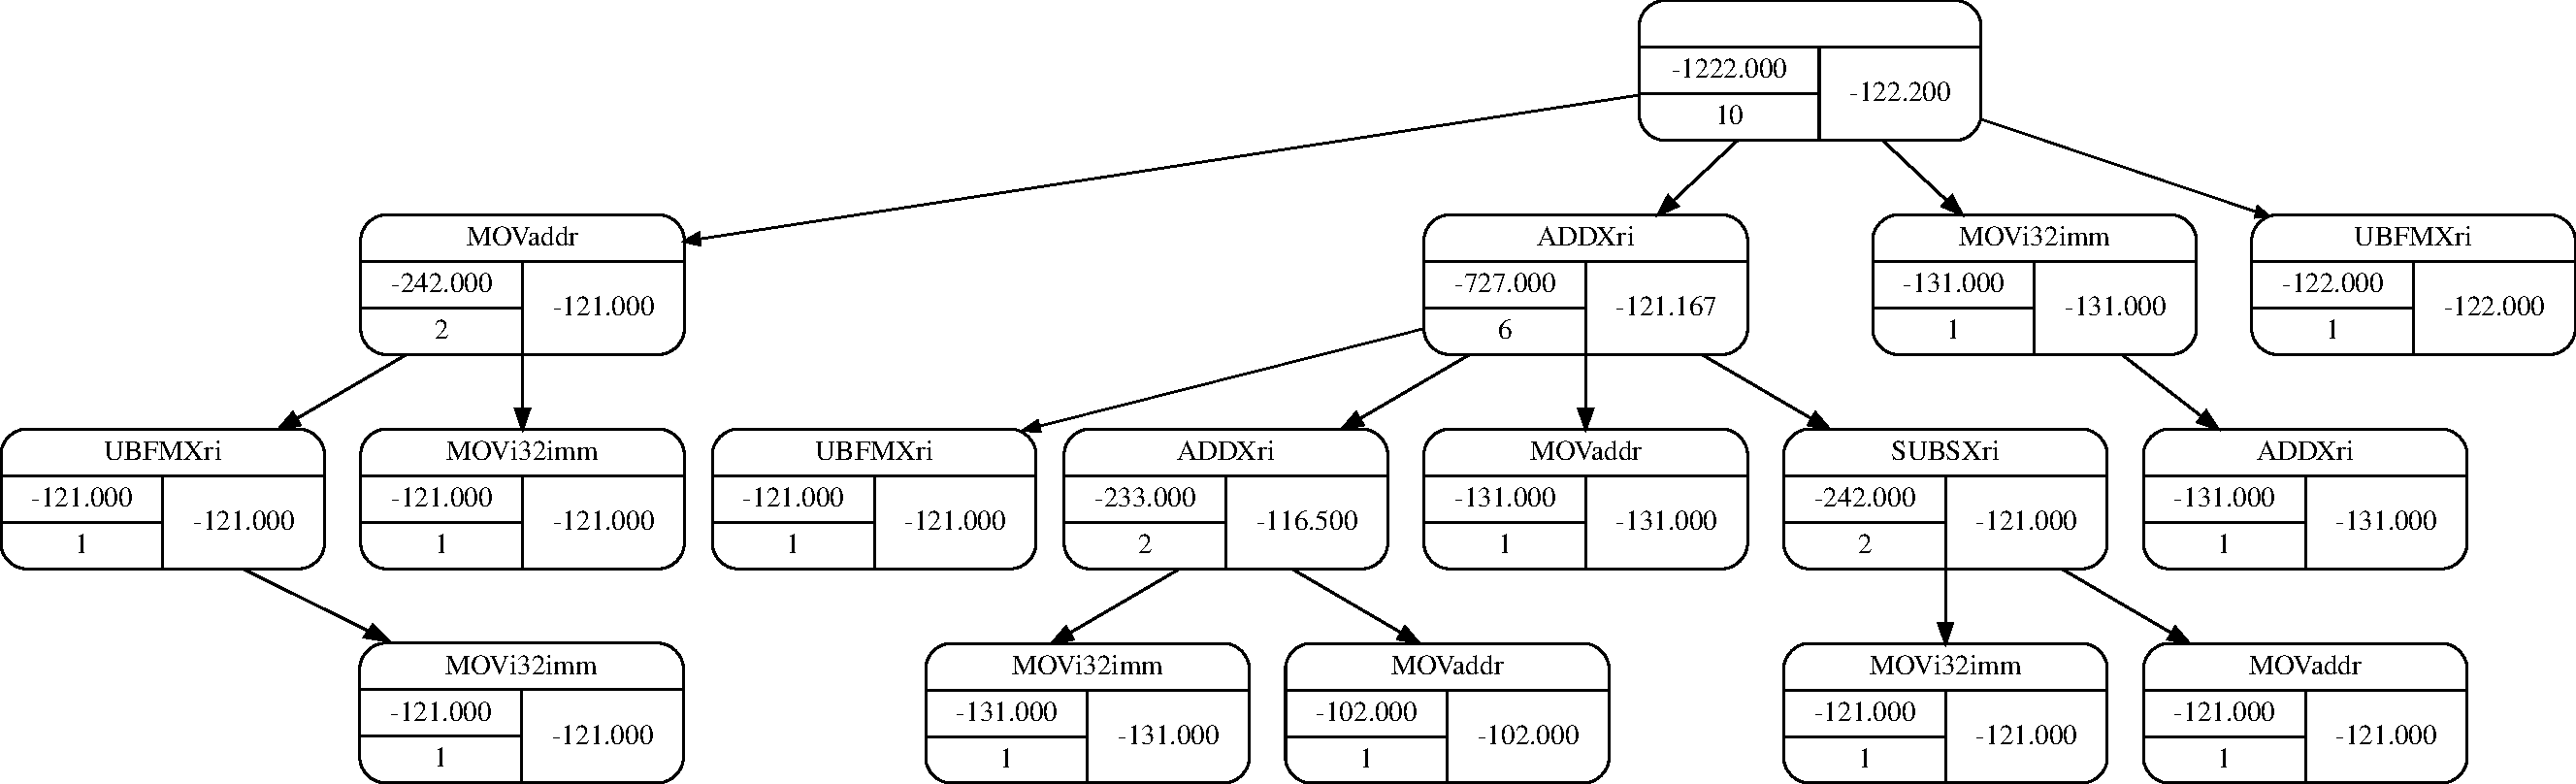
\includegraphics[width=18cm,angle=90]{data/mcts-max-vs-avg/svg/selected/8752639012199.pdf}
        \caption{\ac{mcts} tree}
        \label{fig:approach:max-vs-avg:a}
    \end{subfigure}
    \hspace{0.2\textwidth}
    \begin{subfigure}[b]{0.3\textwidth}
        \centering
        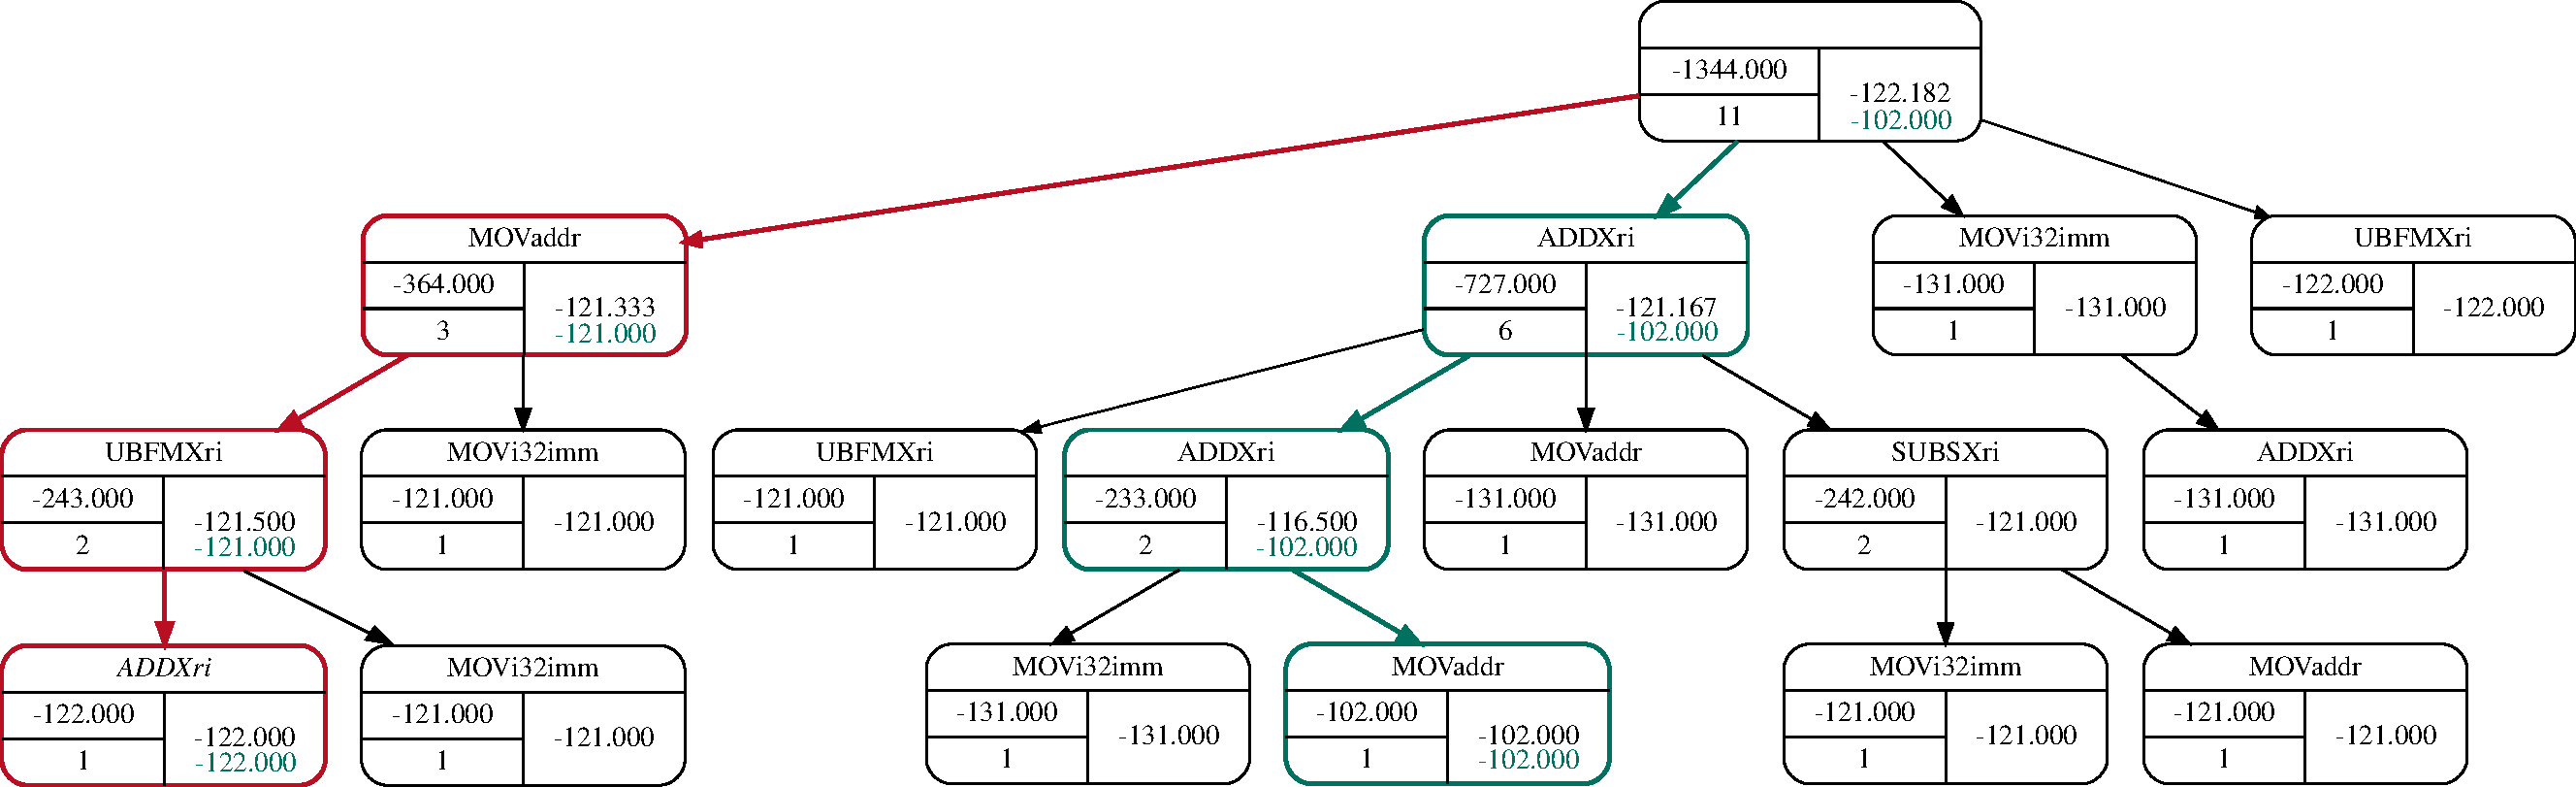
\includegraphics[width=18cm,angle=90]{data/mcts-max-vs-avg/svg/selected/8752639012199-next.pdf}
        \caption{\ac{mcts} tree after next iteration}
        \label{fig:approach:max-vs-avg:b}
    \end{subfigure}
    \caption[\ac{mcts} tree with the consequences of maximum and average metric]{
        \Cref{fig:approach:max-vs-avg:a} shows a given \ac{mcts} tree and \cref{fig:approach:max-vs-avg:b} shows two different choices on different \ac{mcts} metrics.
        The boxes represent a \ac{mcts} node, at the top is the name of the instruction, on the left are the cumuluated metric and the number of visits, on the right is the reduced metric.
        In this example, the value used for the metric is the negative runtime, because we try to maximize the metric.
        The red path is chosen when we used the average metric. But if we choose the maximum metric (green path) we can see, that we find a better runtime.\\
        (Benchmark: LoopRestructuring-dbl, Function: s2233, Basic Block: for.body20)
    }
    \label{fig:approach:max-vs-avg}
\end{figure}

We do not use the default choice of node evaluation metric.
Typically, to evaluate the reward of a node in the \ac{mcts} tree, you compute the average of the children nodes.
In our approach, this leads to situations where we have already found a good schedule but keep searching for schedules in another area of the tree.
The reason for that is that the good schedule might be surrounded by relatively bad schedules, which have a negative effect on the average evaluation.
When you train \ac{mcts} for games, that makes sense because you do not want to get into situations where only one good state exists, and the surrounding ones would let you lose the game.
But we are only interested in a single best schedule, therefore we do not care about similar but bad schedules.
The consequence is that we do not take the average but the maximum.
This means that in the exploitation phase, we always follow the path to the best-found schedule.
You can observe the consequences in \cref{fig:approach:max-vs-avg:b}, where the green numbers represent the maximum metric and the black numbers represent the average metric.

% Explain process: Generate schedule -> compile -> measure runtime -> train mcts -> go to 1
The \ac{mcts} learning process is separated into four phases:
\begin{enumerate}
    \item Generate schedule: \\
    Apply the exploration or exploitation phase and generate a new schedule based on our previous experience.
    \item Compile the generated schedule: \\
    The generated schedule is transformed into a C++ file with a function that contains the inline assembly of the scheduled basic block.
    We then compile the schedule with our benchmarking framework (see \cref{sec:approach:isol_bb_exec}).
    \item Execute and measure the runtime: \\
    The compiled executable is transferred to our target machine and executed there to measure the runtime of the basic block (see \cref{sec:approach:isol_bb_exec}).
    \item Progress the \ac{mcts} tree with the measured runtime: \\
    Then, the measurement data is copied back to the machine where we run the experiment.
    The measurement data is preprocessed and used to train the \ac{mcts} tree.
\end{enumerate}
This process is repeated many times, depending on the experiment.
See \cref{sec:bg:mcts} for more information.

% Technically possible to use for production, but slow
Note that this \ac{mcts} approach is not only able to generate data for our global model.
It can theoretically also be used in a normal compilation process.
It is not practical to use it for a whole program because of the many compilation steps and the bad runtime performance.
But critical parts of a program could be optimized with this approach.

% Positive sideeffect: Also there to define a possible range of improvement
A positive side effect of this \ac{mcts} approach is that we generate an upper limit for the improvements of the instruction scheduling phase.
This is at the same time an upper limit for the global models in our second step.
Therefore, we can see how much of our potential improvements we are able to reach with our global models.

\subsection{Global Model}
\label{subsec:approach:ml:global}
Once we have found good schedules by generating \ac{mcts} trees for many basic blocks, we want to generalize this knowledge.
This is necessary to transfer the knowledge to unseen basic blocks and make the model usable in practice by generating good schedules directly, in contrast to searching them with \ac{mcts}.
Therefore, we have developed three different models that we discuss here.

\subsubsection{Look-Up Model}
Our first model involved no complex algorithms but only searched for similar scheduling situations.
That means we search our \ac{mcts} trees and build up a big model in which we can search for situations and see what decision performed best.

% Dataformat: (h_n, ..., h_1) x (i_1, i_2) -> (w_1, d, w_2)
In order to build the model, we first define the data that we want to save and want to access.
A scheduling situation has the format
\begin{equation}
    (h_n, \ldots, h_1) \times {i_1, \ldots, i_m}
    \label{eqn:approach:example-scheduling-situation}
\end{equation}
where instructions $h$ build a sequence of last scheduled instructions and instructions $i$ build the set of available instructions for scheduling.
To simplify our model and have more data per scheduling situation, we limited the size of the set of available instructions to two.
The disadvantage is that we lose some context information on which other instructions are available.
The data we are interested in per scheduling situation is how often instruction $x$ was better than instruction $y$ or vice versa and or often they were equally good.
This results in the data format
\begin{equation}
    (h_n, \ldots, h_1) \times (i_1, i_2) \mapsto (w_1, d, w_2)
\end{equation}
where $w_1$ and $w_2$ represent how often instruction $i_1$, or $i_2$ was the better choice.
How often they were equally good is counted by the variable $d$.

% How to build this model?
To build the model, we iterate the \ac{mcts} trees and extract the contained data.
\begin{figure}
    \centering
    \begin{forest}
        [$h_n$
            [$\vdots$
                [$h_1$
                    [$i_1$] [$i_2 $] [$i_3$]
                ]
            ]
        ]
    \end{forest}
    \caption[Example scheduling situation]{Example scheduling situation with the already scheduled instructions $h$ and the instructions $i$ to choose from.}
    \label{fig:approach:example-scheduling-situation}
\end{figure}
For every scheduling situation (compare \cref{eqn:approach:example-scheduling-situation} and \cref{fig:approach:example-scheduling-situation}), we take every combination of instructions $i$.
For each combination, we check which instruction choice resulted in a better reward.
We add this situation to our model if it was not already present.
Otherwise, we increase the corresponding counter variable in this situation.

In addition to this situation, we can also learn from this situation for a scheduling situation with a shorter history.
So we also add the situation for all partial histories.
For example, when we have a scheduling situation with the history $(h_3, h_2, h_1)$, we also add our learnings to the model with the histories $(h_2, h_1)$, $(h_1)$, and the empty history $()$.

% How to make scheduling decisions from this model?
This model can be easily applied for scheduling.
In a given scheduling situation, we just search for the history and all combinations of available instructions.
If we have found all the combinations, we can make our decision based on the counts.
For the situation where we did not find all the required combinations, we define a percentage threshold $t_c$.
If we found more than $t_c$ instruction combinations, we make a choice based on the instructions that we have found.
If we found fewer than $t_c$ instructions, we remove the oldest instruction $h_n$ from the history and search again for all the instruction combinations. 

\subsubsection{Support Vector Machine Model}
% What mapping are we trying to learn?
Further, we want to learn regression models.
Therefore, we need a different mapping that we learn because our output will be a scalar value.
\begin{equation}
    (h_n, \ldots, h_1) \times i \times (d_{min}, d_{max}) \mapsto r
    \label{eqn:approach:regression-mapping}
\end{equation}
We choose to have a sequence of history instructions $(h_n, \ldots, h_1)$ with a defined length $n$.
From the history and the choosable instruction $i$ we map to the reward value extracted from the \ac{mcts} data.

One 
\todo{Why exactly did we do this? Pipeline?}
additional metric that we added to our input is, how far in the history the direct \ac{dag} predecessor instructions are scheduled.
For example, instruction $a$ depends on instruction $b$, and we are in the situation in which we want to schedule $a$.
That means we have already scheduled $b$.
There usually also exist other instructions that we scheduled after $b$.
We count the number of instructions that we scheduled between $a$ and $b$.
There are typically more than one instructions that $a$ depends on, so we decided to take the maximum and the minimum number of instructions between $a$ and its predecessors for the dataset.
We refer to these values as $d_{max}$ and $d_{min}$ in \cref{eqn:approach:regression-mapping}.

% How was the input data generated?
To build a dataset with the mapping defined in \cref{eqn:approach:regression-mapping} we iterate the \ac{mcts} trees, and for every instruction node, we take its past scheduled instructions and the reward value it has.
This way, we collected 4.8 million data points for the AARCH64 architecture.
\todo{Add number for aurora}

% Data preprocessing
However, we cannot insert these data points into the \ac{svm} model because it requires numerical values only.
We transform the instructions from their textual representation into an ordinal encoding, \ie every instruction gets a unique numerical representation.
Further, we scale all numerical values into the range $[0,1]$ because \acp{svm} typically learn better when inputs are in this range.

With this data, we train an \ac{svm} regression model.
The details and results of the experiments can be found in \cref{eval:svm}.

\subsubsection{Neural Network Model}
We chose to use a neural network as a second regression model.
With this mode, we try to learn the same mapping as we did with our \ac{svm} model, which is defined in \cref{eqn:approach:regression-mapping}.
Consequently, we use the same dataset that we have already built for the \ac{svm} model.

In contrast to our \ac{svm} model, we chose not to encode the instructions into ordinary values.
The instructions are encoded into one-hot vectors because neural networks can better handle high-dimensional inputs.
Further, the scaling of numerical values into the range $[0,1]$ is also done in this case.

We trained a neural network with this data setup but also tried a modification.
To reduce the dimensionality of the data, we clustered similar instructions.
Especially instructions that only vary in the number of bits in the inputs.
The addition instructions \lstinline|ADDWri| and \lstinline|ADDXri| of the AARCH64 architecture are clustered into the same cluster.
These two instructions only differ in that one takes 32-bit values and the other 64-bit values.
\todo{Add clusterings into appendix}
See \cref{tab:xxx} for exact clusterings.

\section{Data Generation}
\tobechecked
We cannot build our data-driven models (see \cref{sec:approach:ml}) directly from our dataset, described in \cref{sec:approach:dataset}.
Learning from this dataset requires some transformation from the code to a metric we are interested in.
Many metrics can be chosen for optimization, \eg runtime, energy consumption, cache misses, processor stalls.
We focus on optimizing the instruction scheduling for short runtimes.
To generate data for our MCTS approach, we need a mapping from instruction schedules to runtimes.

The most reliable approach is to measure the runtime while executing the code.
\todo{Discuss these in related work. Check Ithemal paper for more ressources}
However, research on approaches that rely on analytical models exists~\cite{llvm:mca, mendis2019ithemal, taha2003instruction, laukemann2018automated}.
We will choose the classical approach of runtime measurements since we have access to the hardware, and the resulting data will be more accurate.
Therefore, we compile the code with varying instruction schedules and execute it to measure its runtime.
We discuss various aspects of this in the remainder of this section.

\begin{figure}
    \centering
    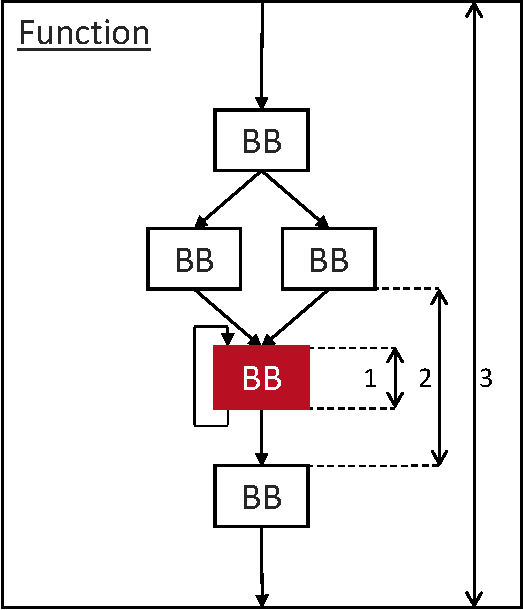
\includegraphics[scale=0.8]{img/ppt/runtime_measurement_scopes-crop.pdf}
    \caption[Possibile scopes for measuring runtimes]{The outer box represents a function. 
    The function consists of multiple basic blocks (BB) where different possible branches are caused by if/else statements and loops. 
    The diagram shows three possible runtime measuring scopes to measure the runtime of the filled basic block.
    Method 1 shows a measuring inside of a basic block. 
    With method 2, the measurement starts with the end of the last basic block and ends with the start of the next one.
    Method 3 measures the complete function which surrounds the basic block.}
    \label{fig:approach:runtime_scopes}
\end{figure}

\subsection{Runtime Measurement Unit}
\tobechecked
The metric we are interested in specifically is the relative runtime compared to a baseline runtime.
Runtime overheads can be ignored in our approach, as long as they are constant over multiple runs.
Thus, various possibilities for placing the start and stop events of the timer exist to accomplish runtime measurements of fractions of the application's code.
The objective is to minimize noise and get reliable, reproducible measurements.
We discuss the possibilities of making measurements on a basic block, function, and application scope and relevant aspects to these possibilities.

\subsubsection{Application}
\tobechecked
\label{sec:approach:datageneration:runtime:app}
The most straightforward approach to measuring the runtime of a piece of code is to measure the runtime of its whole application.
The disadvantage is that we include many more instructions in the measurement than we are interested in.
This generates lots of noise from various possible sources (\eg from \ac{io} instructions like opening files, printing to the screen, or varying latencies for memory accesses).
Also, the longer the runtime of a program, the higher is the probability that the operating system will interrupt the execution for more important processes.
Depending on the used measurement method (see \cref{sec:approach:datageneration:runtime_methods}), this will be included or not be included in the measurement.
These disadvantages make this approach unreliable and not usable for us because we are interested in the short runtime of a single basic block.

\subsubsection{Function}
\tobechecked
\label{sec:approach:datageneration:runtime:function}
A finer-grained approach is to start the timer at the beginning of the function or method that contains the basic block of interest and stop the timer at the end of the function (see method 3 in \cref{fig:approach:runtime_scopes}).
There come several problems with this approach.

Compared to measuring the runtime of the whole application (see \cref{sec:approach:datageneration:runtime:app}), this approach executes only a small fraction of the code.
This results in a lower probability for variances in the measured runtimes due to fewer \ac{os} interruptions, and fewer memory and \ac{io} accesses.
Thus, the precision of these measurements is higher.

Notice in \cref{fig:approach:runtime_scopes} that there are different control paths are possible in a function, based on if/else statements or loops.
This can be problematic in a general setup.
However, the benchmarks we use and the data we insert to them are deterministic, \ie the same paths are taken with each benchmark execution.
Theoretically, if there were no variance in the measurements, the shortest measured execution time would always correspond to the same execution path.
In practice, we get many varying measurements because of different execution paths.
That makes it difficult to differentiate between execution paths and variance in the measurements.

\subsubsection{Basic Block}
\tobechecked
The most intuitive approach is to measure only the runtime of the basic block we are interested in.
We eliminate all extra processor instructions that we are not interested in.
However, we can still get runtime variations for different reasons:
\begin{itemize}
    \item The basic block could call other functions which could execute varying branches. 
          See \cref{sec:approach:bbisolation} for a discussion about this.
    \item The \ac{os} could interrupt the execution. 
          But the probability decreases with shorter code fragments.
\end{itemize}

One requirement that can not be met in all situations is that we require a very precise timer.
These timers usually depend on the hardware directly, \ie the hardware must provide such functionality to measure runtimes.
This is possible on our chosen hardware and is discussed in more detail in \cref{sec:approach:hwpercounter}.

Thus, as this is a feasible solution for our experiments, we have chosen to measure the runtime of basic blocks alone.
    
\subsection{Runtime Measurement Methods}
\tobechecked
\label{sec:approach:datageneration:runtime_methods}
% \todo{Could add little experiment where we compare hardware timers vs OS access}
Various possibilities to observe execution times exist in systems that we are using for our research.
These can typically be classified into the categories of profiling, \ac{os} utilities, or hardware utilities.
We discuss these here in more detail.

\subsubsection{Profiling}
\tobechecked
Profilers are programs that observe the execution of other processes running on the system (\eg gperf \cite{graham1982gprof}).
They are designed to observe the execution from start to end and to return various metrics. Some examples are:
\begin{itemize}
    \item execution times per function
    \item memory consumption
    \item cache misses
\end{itemize}
The observation is done by doing snapshots of the process of interest.
Thus, profilers are good for finding, \eg performance problems and memory leaks in software.

However, we need precise measurements from instruction A to instruction B for our experiments.
Profilers are not able to make such precise measurements, \ie they are not helpful to us because they are designed for other purposes.

\subsubsection{Operating System Methods}
\tobechecked
\acp{os} typically need to work with times and also provide a user interface to use its timing functions.
These are using some \ac{cpu} functionality to get times.
However, often there are various possibilities to retrieve timing values from the hardware with varying precision.
The most precise timers are usually good for measuring intervals in the microseconds range or longer.
The \ac{os} functions have some overhead because they also handle errors.
\begin{table}
    \centering
    \begin{tabular}{@{}ll@{}}
        \toprule
        Operating System & Timer in C language \\
        \midrule
        Linux & \lstinline|clock_gettime()| \\
        Windows & \lstinline|QueryPerformanceCounter()| \\
        \bottomrule
    \end{tabular}
    \caption[Operating System interfaces to their timing functions]
    {
        The table shows examples for interfaces in \acp{os} to their timing functions in the C programming language.
    }
    \label{tab:approach:timing_functions}
\end{table}
See \cref{tab:approach:timing_functions} for selected \acp{os}.
The C++ function \lstinline|std::high_resolution_clock()| from the standard library falls back to one of these \ac{os} functions.

\acp{os} sometimes not only provide timing methods but also allows us to manage how a process will be executed.
Linux provides different methods to avoid or reduce the probability of \ac{os} interrupts during the execution of a process.
\begin{itemize}
    \item Isolating \ac{cpu} cores: 
    The Linux kernel command line option \lstinline|isolcpus=[cpu_number]| in the boot loader instructs Linux to not schedule tasks to the given \ac{cpu} cores automatically.
    \item Pinning a process to a \ac{cpu} core: 
    The Linux program \lstinline|taskset| can specify on which \ac{cpu} core a process will be scheduled.
    This can also be used to schedule processes on isolated \ac{cpu} cores.
\end{itemize}
When we pin a process to an isolated \ac{cpu} core, this task will not be interrupted by the \ac{os}.
This makes the measuring of runtimes more reliable.

\subsubsection{Hardware Performance Counters}
\tobechecked
\label{sec:approach:hwpercounter}
The most code blocks we want to measure are only 5-50 instructions long, \ie we need very precise measurements.
We use the assembly instructions of the given hardware directly to get the most precise timing values with the lowest overhead.
These instructions typically return the value of a processor cycle counter register.

Using assembly instructions can be complicated (depending on the used high-level language and hardware).
But it is not a problem in our experiments because the code blocks we want to measure are already written in the assembly language of the given hardware.
That means we only add a timer instruction at the beginning and one at the end.
We do some error checking after the execution has stopped (see \cref{sec:approach:isol_bb_exec} for details).
\begin{table}
    \centering
    \begin{tabular}{@{}ll@{}}
        \toprule
        Hardware & Assembly instruction \\
        \midrule
        x86 & \lstinline|rdtsc| \\
        ARM32 & \lstinline|mrc p15m, 0, r0, c15, c12, 1| \\
        AARCH64 & \lstinline|mrs x0, PMCCNTR_EL0| \\
        NEC SX-Aurora TSUBASA & \lstinline|smir %s60, %usrcc| \\
        \bottomrule
    \end{tabular}
    \caption{Assembly instructions for getting the cycle counter value of a given hardware.}
    \label{tab:approach:asm_instrs_timing}
\end{table}
See \cref{tab:approach:asm_instrs_timing} for the assembly instructions per hardware.

Depending on the hardware and the \ac{os}, access to these instructions or registers might not be permitted.
For the AARCH64 architecture and a Linux \ac{os}, we had to implement and load a kernel module that granted access to this register.
 

\subsection{Execution Unit}
% \todo{Provide runtime example data}
\label{sec:approach:exec_unit}
For the learning process, we have to execute the differently scheduled basic blocks many times.
This can be time-intensive, and many lines of code are executed that we are not interested in.
The scope of the thesis forces us to extract the basic block from the benchmark and execute it in isolation.
Here, we discuss the advantages and disadvantages of the two possible approaches.

\subsubsection{Benchmark}
The first option is to execute the complete benchmark for every new schedule that was generated during the learning process.
The advantage is that we execute the original basic block as it would appear in the real benchmark.
The problem with this approach is that the execution time of a benchmark can be high and makes the execution the bottleneck in our pipeline.
Many benchmarks in our dataset take several minutes to execute on a RaspberryPi 3B.
So, always executing the whole benchmark is costly to even get only one runtime measurement per schedule.
In order to get statistically relevant runtimes, we have to measure them multiple times.

\subsubsection{Basic Block}
The alternative to executing the whole benchmark is to extract the scheduled basic block from the benchmark and execute it in isolation.
By using this approach, we reduce the execution time to a minimum and do not execute code we are not interested in.
Consequently, we can execute the benchmark many times and get statistically reliable runtime measurements.
The disadvantage is that we have to slightly modify the basic block or the program will crash.

\subsection{Basic Block Isolation}
\label{sec:approach:bbisolation}
As discussed in \cref{sec:approach:exec_unit}, we are forced to execute basic blocks isolated from the benchmark.
To make a basic block executable, we isolate it and insert it as inline assembly into our minimal C++ framework.

\subsubsection{Basic Block Extraction}
% \todo{include numbers on speedup vs. benchmarking full function}
First, we compile the benchmark and schedule the basic block with our modified compilation process (see \cref{sec:approach:build_process}) into assembly files.
Next, we extract the basic block instructions from the assembly file.
Then, we modify the basic block instructions slightly to prevent execution and compilation errors, and as the last step, we inject it into our C++ framework.

The assembly code can contain some lines that will make our framework crash.
We are forced to modify or delete these lines.

Assembly files contain comments, labels, and assembler directives which will be removed.
Comments are useless lines for the execution task. 
The labels are not required, as we will not jump to other instructions.
And assembler directives represent commands to the assembler program for bookkeeping, storage reservation, and other purposes.
These could interfere with our compilation process and are also removed.

Basic blocks can contain jump instructions as the last instruction and function calls in any position.
We only schedule the instructions in the given basic block, so we are also only interested in its own runtime.
Executing other code, which could internally choose different paths, would add noise to our measurements.
To prevent this uncontrolled program execution, we simply remove jump and call instructions.
The removal of these instructions might slightly reduce the execution time, but the reduction is constant over all executions with different schedules.

In order to prevent segmentation faults, we have to redirect all memory accesses to a memory area that we are allowed to read and write to.
This affects all load and store instructions.
In our framework, we allocate 8 byte on the stack where we redirect all memory accesses.
This also means that all memory accesses are cache hits, and we have a controlled environment in this aspect.

\todo{Show example}

\subsubsection{Isolated Basic Block Execution}
\label{sec:approach:isol_bb_exec}
\tobechecked
To execute the extracted basic block, we have to surround it with some other code to generate a valid C/C++ program.
For this, we have written a small benchmarking framework.
This framework is compiled together with the given basic block in the inline assembly format.
The optimization is turned off in this compilation step, so the basic blocks are executed as given.

The executable first executes the basic block in 100 warmup rounds to prevent side effects from caches and other reasons.
The actual execution where we measure the runtime is repeated until 1,000 valid measurements are done.
Invalid measurements can occur when the runtime is negative.
This happens when the cycle counter overflows.

\subsection{Computing Rewards From Runtimes}
\tobechecked
Even though we do the warmup rounds, we still get few data points that are clearly outliers and should not be included in our experiments.
We sort the 1,000 runtime measurements and strip the top and bottom 50 measurements.
Spot checks have shown that we remove all the outliers in almost all the experiments.
\begin{table}
    \centering
    \begin{tabular}{@{}rr@{}}
        \toprule
        Runtime & Num. Occurances \\
        \midrule
        140 & 998 \\
        143 & 1 \\
        711 & 1 \\
        \bottomrule
    \end{tabular}
    \hspace{0.8cm}
    \begin{tabular}{@{}rr@{}}
        \toprule
        Runtime & Num. Occurances \\
        \midrule
        121 & 708 \\
        120 & 289 \\
        123 & 1 \\
        163 & 1 \\
        1491 & 1 \\
        \bottomrule
    \end{tabular}
    \hspace{0.8cm}
    \begin{tabular}{@{}rr@{}}
        \toprule
        Runtime & Num. Occurances \\
        \midrule
        114 & 994 \\
        121 & 2 \\
        115 & 1 \\
        129 & 1 \\
        130 & 1 \\
        694 & 1 \\
        \bottomrule
    \end{tabular}
    \caption[Example runtime measurement distribution]{Example runtime measurement distribution for three different schedules. (Benchmark: almabench, Function: anpm, Basic Block: entry)}
    \label{tab:approach:example_runtimes}
\end{table}
See \cref{tab:approach:example_runtimes} for an example with three different schedules for the same experiment.

Because different basic blocks have their different runtimes, the absolute measured speedups between two basic blocks are not comparable.
To have a metric $m$ that we can compare with all other basic blocks in the data set, we normalize the experiment runtime $r_e$ with the runtime of the baseline scheduler $r_b$.
\begin{equation}
    m=\frac{r_b}{r_e}
\end{equation}

\section{Application of the Learned Model}
\label{sec:approach:ml-scheduler}
\todo{Write about how we run the learned models and how we make measurements}
